\documentclass[a4paper,12pt]{article}
\usepackage[utf8]{inputenc}
\usepackage[T1]{fontenc}
\usepackage[french]{babel}
\usepackage{lmodern}
\usepackage{hyperref}
\usepackage{bookmark}
\usepackage{graphicx}
\usepackage{listings}
\usepackage{xcolor}
\usepackage{amsmath}

\usepackage{amsfonts} % Pour \mathbb{P}

\lstset{
    language=JavaScript,
    basicstyle=\ttfamily,
    keywordstyle=\color{blue},
    stringstyle=\color{red},
    commentstyle=\color{green},
    morecomment=[s][\color{magenta}]{/*}{*/},
    breaklines=true
}

\title{\textbf{Apprentissage des Protocoles de Communication pour les Algorithmes Distribués}}
\author{}
\date{}

\begin{document}

\maketitle
\newpage

\tableofcontents
\newpage

\section{Introduction}
Les algorithmes distribués jouent un rôle fondamental dans la gestion et l'analyse des réseaux à grande échelle. Dans le modèle LOCAL, chaque nœud d’un graphe ne communique qu’avec ses voisins immédiats pour résoudre un problème global tout en minimisant le nombre de tours de communication. Toutefois, la communication représente souvent un goulot d’étranglement dans ces algorithmes, et la défaillance d’un ou plusieurs nœuds peut perturber considérablement le processus. 

L’objectif de ce travail est d’explorer comment les techniques d’apprentissage automatique peuvent être utilisées pour prédire les bits transmis par les nœuds voisins dans un contexte distribué. Cela permettrait de remplacer les informations manquantes et d’assurer une plus grande robustesse des algorithmes contre les pannes.

\section{État de l’Art}
Les algorithmes distribués classiques tels que le MIS (Maximal Independent Set) et le Graph Coloring fonctionnent en minimisant les communications tout en assurant l’optimisation des résultats globaux. Cependant, ces algorithmes sont vulnérables aux pannes des nœuds et nécessitent des stratégies avancées pour la gestion des erreurs.

Les approches existantes utilisent principalement des techniques de redondance ou de recalcul partiel, mais elles restent coûteuses en termes de ressources. L’intégration de l’apprentissage automatique pourrait apporter une alternative plus efficace en prédisant les communications perdues.

\section{Modélisation du Problème}
Nous avons défini notre problématique principale autour des questions suivantes :
\begin{itemize}
    \item Comment prédire les bits de communication échangés entre nœuds ?
    \item Quels modèles d’apprentissage sont les plus efficaces pour cette tâche ?
    \item Comment intégrer ces modèles dans un environnement distribué avec des contraintes de temps réel ?
\end{itemize}


\section{Algorithme Alice--Bob}

Dans le modèle classique d'un réseau pair-à-pair (P2P), deux nœuds -- nommés Alice et Bob -- échangent des bits (0 ou 1). Cependant, l'un des deux (par exemple, Bob) peut se déconnecter à tout moment et cesser d'envoyer de nouveaux bits. Dans ce cas, l'autre nœud (Alice) doit deviner les bits que Bob aurait pu envoyer. Étant donné que ces bits sont générés de façon aléatoire (avec une probabilité \texttt{p\_one} d'être égaux à 1), il est impossible de les prédire parfaitement.

\subsection{Problématique principale}
L'objectif est de minimiser l'erreur de transmission malgré cette
déconnexion. Chaque nœud maintient un historique des bits récents reçus sous forme d'un tampon (buffer). Quand un nœud se déconnecte, l'autre tente de prédire les bits manquants grâce aux statistiques de son buffer. L'aspect aléatoire de la génération des bits entraîne inévitablement une incertitude dans la prédiction, mais cette méthode permet de poursuivre la simulation ou la communication sans interrompre complètement le processus.

\subsection{Paramètres et implémentation du code}
Chaque nœud (Alice ou Bob) est caractérisé par :
\begin{itemize}
  \item \texttt{p\_one} : la probabilité d'envoyer un bit valant 1.
  \item \texttt{buffer\_size} : la taille du buffer pour stocker
        les bits récemment reçus.
  \item \texttt{is\_disconnected} : un indicateur booléen précisant
        si le nœud est déconnecté.
  \item \texttt{count\_ones} et \texttt{count\_total} : le décompte
        de bits 1 et le nombre total de bits reçus, utiles pour
        calculer une probabilité de prédiction.
\end{itemize}

Lorsqu'un nœud est déconnecté, il ne peut plus envoyer de bits, et l'autre nœud doit appeler une fonction de \og devinette \fg{} (guess). Ci-dessous, nous présentons uniquement les deux méthodes principales pour envoyer et deviner un bit :

\paragraph{Extrait de code pertinent :}
\begin{verbatim}
# --- Création du message ---
def send_message(self):
    if self.is_disconnected:
        return None
    bit = 1 if random.random() < self.p_one else 0
    return bit

# --- Devinette du message ---
def guess_message(self):
    if self.count_total == 0:
        return 0
    if self.count_total >= self.buffer_size:
        prob_one = self.count_ones / self.buffer_size
    else:
        prob_one = self.count_ones / self.count_total
    return 1 if random.random() < prob_one else 0
\end{verbatim}

\subsection{Conclusion et brève allusion aux travaux futurs}
Cet algorithme classique montre comment gérer la déconnexion éventuelle d'un nœud dans un réseau P2P en conservant un estimé des bits manquants. Certes, la précision n'est pas garantie en raison de l'aléatoire inhérente à la génération des bits, mais cette approche maintient la cohérence des échanges et évite l'arrêt brutal de la communication. Enfin, on peut noter qu'une étape ultérieure consistera à calculer et analyser la quantité de données perdues (\emph{miss}) et à mettre en place des méthode plus avancées pour la reconstruction des données manquantes, si nécessaire.



\section{Algorithme Alice--Bob}
Dans un réseau pair-à-pair (P2P) où chaque nœud génère aléatoirement des bits (0 ou 1) avec une certaine probabilité $p_{\text{one}}$, l’algorithme Alice--Bob sert à gérer les déconnexions soudaines des nœuds. Lorsque Bob se déconnecte, Alice essaie de deviner les bits que Bob aurait envoyés. Dans la version \textit{classique}, cette prédiction se base simplement sur la proportion de 1 reçus dans le buffer (méthode \texttt{guess\_message}). Cependant, nous proposons ici une version améliorée où Alice utilise un modèle de \textbf{régression logistique} pour prédire les bits manquants.

\subsection{Pourquoi la Régression Logistique ?}

\begin{itemize}
    \item \textbf{Principe de base :}  
    La régression logistique permet de modéliser la probabilité qu’une variable binaire (ici, le bit vaut 1) soit égale à 1 en fonction de certaines variables explicatives (par exemple, l’identifiant de Bob, le nombre de bits déjà reçus, etc.). Elle calcule donc :
    \[
    \mathbb{P}(Y=1 \mid X) = \frac{1}{1 + e^{-(\beta_0 + \beta_1 X_1 + \dots + \beta_n X_n)}}
    \]
    où $Y$ est la variable binaire (le bit), et $X_1, \dots, X_n$ les variables explicatives.

    \item \textbf{Pourquoi utiliser un modèle d’apprentissage ?}  
    \begin{itemize}
    \item \textit{Approche naïve} : On estime la probabilité d’obtenir 1 par $\frac{\text{count\_ones}}{\text{count\_total}}$.
        \item \textit{Régression logistique} : On cherche à faire mieux en exploitant des \textit{features} plus complexes (par exemple, plusieurs Bob, l’historique par Bob, etc.).
    \end{itemize}

    Même si, dans ce projet, les bits sont \textit{effectivement} générés de façon aléatoire selon une probabilité fixe $p_{\text{one}}$, la régression logistique peut s’avérer utile lorsqu’on souhaite tenir compte de plus de paramètres (nombre de déconnexions, contextes, interactions multiples, etc.).

    \item \textbf{Amélioration incertaine :}  
    Dans notre cas précis, puisque la distribution des bits reste purement aléatoire (avec une probabilité fixe), on ne s’attend pas forcément à des gains considérables par rapport à la méthode \textit{compter le nombre de 1 dans le buffer}. Néanmoins, cette approche sert de tremplin pour des scénarios plus complexes ou réalistes (où la probabilité génératrice peut varier avec le temps ou l’environnement).
\end{itemize}

\subsection{Architecture du Code}

\subsubsection{ Héritage : Classe \texttt{Alice} dérivée de \texttt{Node}}

Dans notre implémentation, chaque nœud du réseau (Alice ou Bob) est représenté par la classe \texttt{Node}, qui propose les fonctionnalités de base :

\begin{itemize}
    \item \textbf{Attributs principaux :}
    \begin{itemize}
        \item \texttt{p\_one} : probabilité d’envoyer 1.
        \item \texttt{buffer\_size} : taille du buffer pour stocker les bits reçus.
        \item \texttt{is\_disconnected} : booléen indiquant si le nœud est déconnecté.
        \item \texttt{received\_bits}, \texttt{count\_ones}, \texttt{count\_total} : pour suivre l’historique de bits reçus.
    \end{itemize}

    \item \textbf{Méthodes :}
    \begin{itemize}
        \item \texttt{send\_message()} : envoie un bit en se fondant sur \texttt{p\_one}.
        \item \texttt{receive\_message(bit)} : met à jour le buffer et les compteurs de bits reçus.
        \item \texttt{guess\_message()} : devine un bit lorsqu’un nœud est déconnecté (version de base : probabilité = $\frac{\text{count\_ones}}{\text{count\_total}}$).
    \end{itemize}
\end{itemize}

La classe \texttt{Alice} \textbf{hérite} de \texttt{Node} pour ajouter les capacités suivantes :

\begin{itemize}
    \item \textbf{Attributs spécifiques :}
    \begin{itemize}
        \item \texttt{bob\_history} : dictionnaire pour stocker l’historique par Bob.
        \item \texttt{model} : instance d’un modèle de régression logistique (issu de \texttt{scikit-learn}).
        \item \texttt{training\_data}, \texttt{training\_labels} : pour enregistrer des exemples et entraîner le modèle.
    \end{itemize}

    \item \textbf{Méthodes supplémentaires :}
    \begin{itemize}
        \item \texttt{receive\_message\_from\_bob(bob\_id, bit)} : enregistre les bits reçus de chaque Bob, alimente la base d’apprentissage.
        \item \texttt{train\_model()} : entraîne la régression logistique sur les données recueillies.
        \item \texttt{predict\_message(bob\_id)} : utilise la régression logistique pour deviner le bit manquant d’un Bob déconnecté.
    \end{itemize}
\end{itemize}

\subsubsection{Nouvelle méthode de prédiction (\texttt{guess\_message}) dans la classe \texttt{Alice}}

\begin{verbatim}
def predict_message(self, bob_id):
    """
    Utilise le modèle entraîné pour prédire le bit d'un Bob déconnecté.
    Si le modèle n'est pas encore entraîné, on retombe sur la méthode traditionnelle.
    """
    if not self.is_model_trained:
        return self.guess_message()

    bob_msg_count = len(self.bob_history.get(bob_id, []))
    features = np.array([[bob_id, bob_msg_count]])

    try:
        proba = self.model.predict_proba(features)[0][1]
        bit_prediction = 1 if random.random() < proba else 0
        return bit_prediction
    except Exception as e:
        print(f"Error making prediction: {e}")
        return self.guess_message()
\end{verbatim}

\textit{Remarque :} On conserve la possibilité de repasser par la fonction \texttt{guess\_message} de la classe parente (\texttt{Node}) si le modèle n’est pas (ou mal) entraîné.

\subsection{Performances et Discussion}

\begin{itemize}
    \item \textbf{Pas de gain significatif sur des bits strictement aléatoires :}  
    Les bits envoyés par Bob sont générés selon une loi de Bernoulli de paramètre $p_{bob}$. Par conséquent, la régression logistique ne trouve pas de corrélations notables, aboutissant à des performances proches de la méthode naïve.

    \item \textbf{Maintien des nœuds déconnectés :}  
    Les nœuds “fantômes” restent pris en compte dans les prédictions. Cette politique permet de réintégrer un nœud si celui-ci revient en ligne, en conservant son historique.

    \item \textbf{Prochaines étapes :}
    \begin{itemize}
        \item Reconstruction de bits avec un dataset complexe (MNIST).
        \item Calcul du taux d'erreur (“miss”) et colorisation d’un graphe pour analyser la propagation des erreurs.
    \end{itemize}
\end{itemize}

\subsection{Conclusion}

Dans cette version du rapport, nous avons introduit une extension de l’algorithme Alice--Bob classique, où la prédiction des bits d’un nœud déconnecté s’appuie sur un modèle de régression logistique.  

\textbf{Avantages :}  
Cette approche prouve la faisabilité d’un apprentissage supervisé dans un contexte P2P, avec un code modulaire et extensible.  

\textbf{Limites :}  
Quand les bits sont générés indépendamment et aléatoirement, le modèle ne dispose pas de réelles corrélations à exploiter.  

Ce travail prépare néanmoins l’introduction d’approches plus avancées (autoencodeurs, reconstruction d’images MNIST, calcul du taux d’erreurs “miss”, etc.), cruciales lorsque les données possèdent des structures spatiales ou temporelles plus riches.

\section{Algorithme Alice--MNIST}

Dans cette section, notre objectif principal est de concevoir et de mettre en \oe uvre une approche d'apprentissage automatique pour qu'un réseau pair-\`a-pair (Peer-to-Peer) puisse transmettre efficacement des données d'images et, en cas de perte de certains bits ou pixels, soit capable de reconstruire l'image initiale autant que possible. L'id\'ee directrice est que si, dans un r\'eseau P2P, un pourcentage \'el\'ev\'e de n\oe uds (pixels) se d\'econnectent temporairement, un mod\`ele d'apprentissage puisse estimer les donn\'ees manquantes et reconstituer l'image originale.

\subsection{Problématique}
\textbf{Question principale :}\\
\emph{``Comment exploiter des modèles d'apprentissage automatique pour améliorer la transmission et la reconnaissance de données dans un réseau distribué (Peer-to-Peer) et permettre la récupération de parties manquantes ?''}\\

Ici, nous considérons la situation où un grand nombre de n\oe uds (c'est-à-dire de pixels) sont déconnectés, et le modèle doit estimer au mieux ces éléments manquants en s'appuyant sur les informations restantes.

\subsection{Description}
Dans cet algorithme, nous utilisons le \textbf{jeu de données MNIST}, qui contient des images manuscrites des chiffres de 0 à 9. Ce jeu de données comporte 60\,000 images pour l'entraînement et 10\,000 pour le test. Chaque image est en niveaux de gris (une seule composante) au format 28$\times$28 pixels. Le choix de MNIST est motivé par sa simplicité et sa popularité pour valider des méthodes de reconnaissance d'images.

\subsubsection{Technologies utilisées}
\begin{enumerate}
    \item \textbf{Bibliothèque PyTorch :}\\
    Pour la construction et l'entraînement des modèles d'apprentissage profond (réseaux de neurones convolutifs, etc.).

    \item \textbf{Régression logistique (Logistic Regression) :}\\
    Utilisée dans certaines parties pour estimer la probabilité qu'un bit (ou un pixel) soit 1, au cas où nous n'utiliserions pas l'architecture CNN.

    \item \textbf{Réseau de neurones convolutif (CNN) de type Autoencoder :}\\
    Un CNN est un réseau neuronal conçu pour extraire automatiquement des caractéristiques spatiales d’une image à travers des filtres convolutifs. Un Autoencoder, quant à lui, est un modèle composé d’un encodeur et d’un décodeur, qui apprend à compresser puis reconstruire les données. Dans notre travail, nous utilisons un autoencoder convolutif pour reconstruire les zones manquantes dans les images, en s’appuyant sur les informations partielles disponibles. C'est la partie centrale du modèle pour prédire les pixels déconnectés.

\end{enumerate}

\subsubsection{Pourquoi avoir choisi un CNN et un Autoencoder ?}
\begin{itemize}
    \item \textbf{Représentation compacte (Encodage) et reconstruction (Décodage) :}\\
    Dans le problème de récupération de pixels perdus, un autoencodeur peut prendre en entrée une image partielle (Partial) et produire une reconstruction (Reconstruction) proche de la version initiale.

    \item \textbf{Robustesse face au bruit et aux données manquantes :}\\
    La structure d'un CNN et ses filtres de convolution sont très efficaces pour apprendre les caractéristiques spatiales d'une image, et peuvent assez bien réparer ou compléter les régions détruites ou manquantes.

    \item \textbf{Rapidité et simplicité :}\\
    Les Autoencoders convolutifs sont relativement simples à implémenter pour des données d'image et offrent un bon compromis entre la précision de reconstruction et la rapidité d'entraînement.
\end{itemize}

\subsubsection{Aperçu du code (extraits principaux)}
Voici un exemple de la classe \texttt{CNNAutoencoder}, sans inclure tous les d\'etails afin de ne pas allonger excessivement le rapport :

\begin{verbatim}
class CNNAutoencoder(nn.Module):
    """
    Un autoencodeur convolutionnel simple:
         - Encoder: 2 blocs Conv -> MaxPool
         - Decoder: 2 blocs ConvTranspose
    """
    def __init__(self):
        super(CNNAutoencoder, self).__init__()
        
        # --- Encoder ---
        self.encoder = nn.Sequential(
            nn.Conv2d(1, 32, kernel_size=3, padding=1),
            nn.ReLU(),
            nn.MaxPool2d(2, 2),
            nn.Conv2d(32, 64, kernel_size=3, padding=1),
            nn.ReLU(),
            nn.MaxPool2d(2, 2)
        )
        
        # --- Decoder ---
        self.decoder = nn.Sequential(
            nn.ConvTranspose2d(64, 32, kernel_size=2, stride=2),
            nn.ReLU(),
            nn.ConvTranspose2d(32, 1, kernel_size=2, stride=2)
        )
        
    def forward(self, x):
        encoded = self.encoder(x)
        decoded = self.decoder(encoded)
        return decoded
\end{verbatim}

\noindent
Dans la partie \textbf{Encoder}, on trouve deux couches de convolution suivies de \textbf{MaxPool}, permettant d'extraire et de compresser les caract\'eristiques visuelles de l'image.\\
Dans la partie \textbf{Decoder}, grâce aux couches \texttt{ConvTranspose2d}, on restaure les dimensions originales (28$\times$28).

Les classes comme \texttt{Node} et \texttt{Alice} simulent la logique d'un n\oe ud P2P : gestion de la d\'econnexion (inconnue de l'\'etat d'un pixel) et recours \`a un mod\`ele entra\^in\'e (CNN ou logistic regression) pour deviner les bits manquants. L'essentiel du code se trouve dans le fichier \texttt{p2pmnist.py}.  

La fonction \texttt{train\_cnn\_model\_with\_dynamic\_disconnections(\dots)} illustre la m\'ethode d'entra\^inement : \`a chaque \emph{batch}, un pourcentage de pixels est al\'eatoirement d\'econnect\'e, et le mod\`ele apprend \`a reconstruire l'image malgr\'e cette perte partielle.

\subsection{Résultats}  
Apr\`es avoir entra\^in\'e le mod\`ele sur MNIST en simulant 60\,\% de d\'econnexions, l'Autoencoder a atteint une pr\'ecision moyenne d'environ \textbf{94.7\,\%} dans la pr\'ediction des pixels perdus (calculée comme le pourcentage de bits correctement prédits parmi les pixels déconnectés). De plus, jusqu'\`a \textbf{60\,\% de donn\'ees manquantes}, le mod\`ele parvient \`a reconstruire assez fid\`element la forme g\'en\'erale du chiffre.


\noindent
\textbf{Figure (6-1)} : Voici les \textbf{précisions moyennes} du modèle en fonction de chaque chiffre (de 0 à 9). On observe une précision allant d’environ 92\,\% à 98\,\% selon le chiffre.


\begin{center}
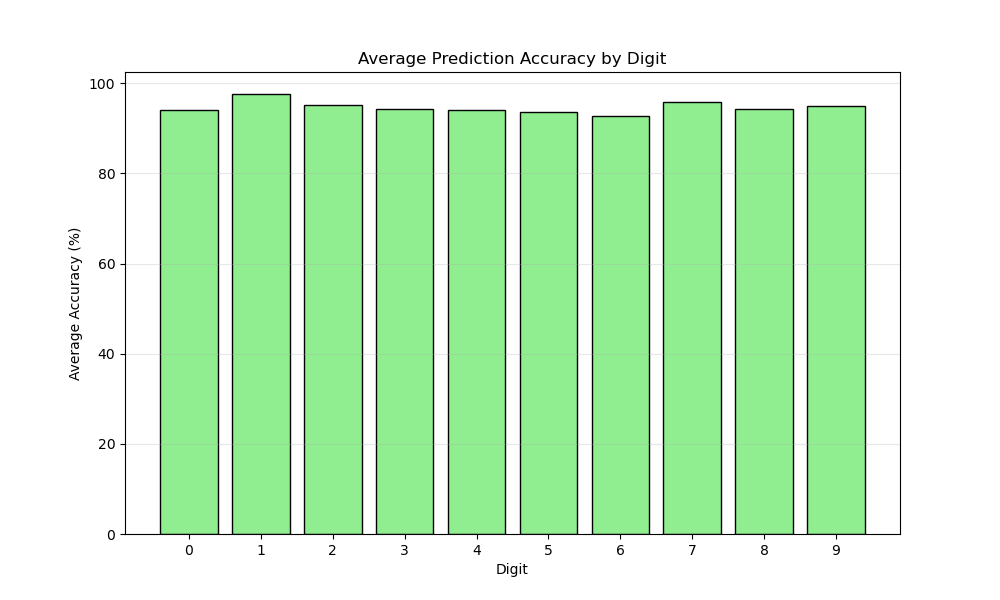
\includegraphics[width=0.9\textwidth]{accuracy_by_digit.png}\\
\emph{Figure (6-1) : Précision moyenne de la reconstruction des pixels manquants pour les chiffres 0 à 9 (en pourcentage).}
\end{center}

\noindent
\textbf{Figure (6--2)} : Elle illustre la distribution des précisions (\emph{Accuracy Distribution}) sur différents échantillons de test. La plupart des échantillons se situent entre 90\,\% et 98\,\% de précision, et la moyenne globale est d’environ 94,79\,\%.

\begin{center}

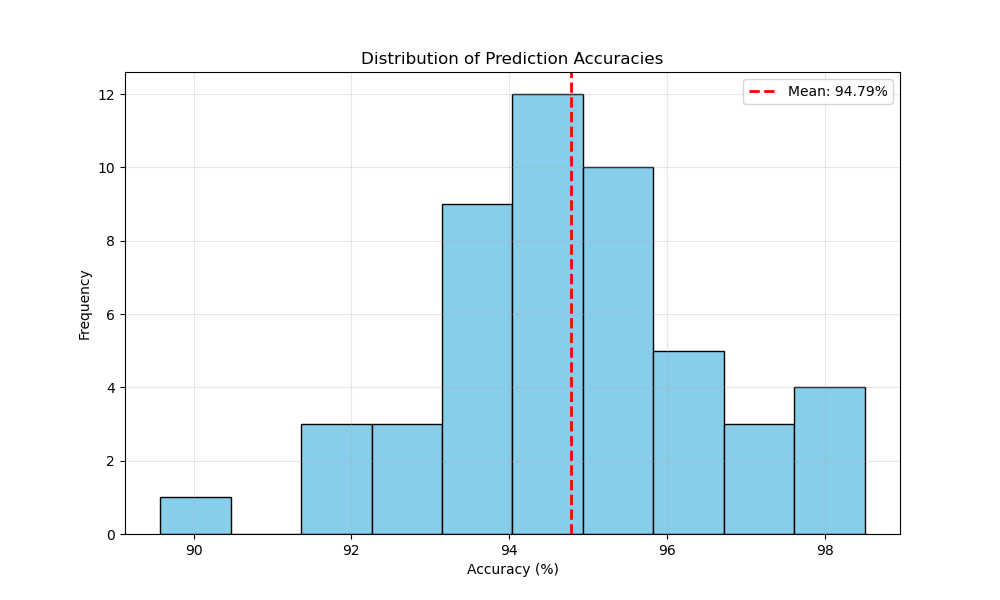
\includegraphics[width=0.9\textwidth]{accuracy_distribution.png}\\

\emph{Figure (6-2) : Distribution de la fréquence de précision de prédiction sur les échantillons de test.}
\end{center}

\noindent
\textbf{Figure (6-3)} : Un exemple concret pour le chiffre «\,5\,» présenté sous trois formes :\\
1. L’image originale (à gauche)\\
2. L’image partielle (au milieu) avec 60\,\% de pixels déconnectés\\
3. L’image reconstruite (à droite) par le modèle, montrant sa capacité à reconstituer l’essentiel du chiffre.

\begin{center}
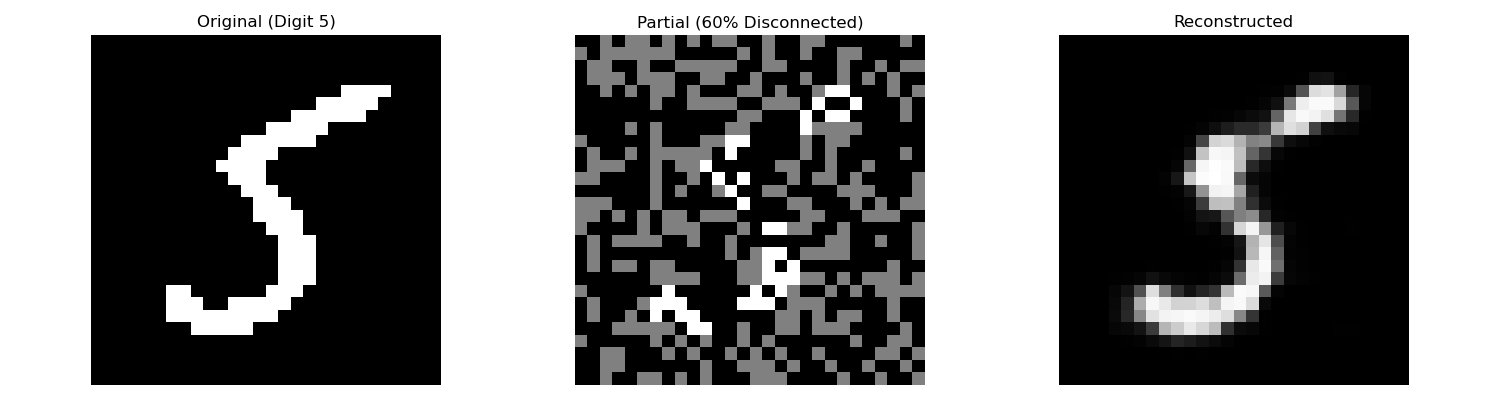
\includegraphics[width=0.9\textwidth]{sample_8.png}\\
\emph{Figure (6-3) : Exemple d'image originale, image avec 60\,\% de pixels déconnectés et image reconstruite par l’Autoencoder.}
\end{center}

\subsection{Limites (Limitations)}
\begin{enumerate}
    \item \textbf{Forte dépendance au type de jeu de données :}\\
    Bien que le modèle fournisse d’excellents résultats sur MNIST (images binaires noir et blanc), dans des cas plus réalistes avec un spectre plus large (images RGB, etc.), il faudra un réseau plus profond et des ensembles de données beaucoup plus volumineux pour reproduire ce type de performance.

    \item \textbf{Besoin de ressources de calcul plus puissantes :}\\
    MNIST est un petit jeu de données relativement simple. Pour obtenir un modèle «\,complet\,» couvrant divers types d'images, il est nécessaire de disposer d'une infrastructure de calcul importante (GPU avancé ou clusters) ainsi que d'ensembles de données massifs.

    \item \textbf{Baisse de performances au-delà de 60\,\% de déconnexion :}\\
    Bien que la reconstruction reste satisfaisante jusqu'à environ 70\,\% de déconnexion pour la majorité des chiffres, on commence à observer une diminution progressive des performances. À partir de 90\,\% de perte de données, le modèle n'arrive plus qu'à reconstruire uniquement le chiffre 1.\\

    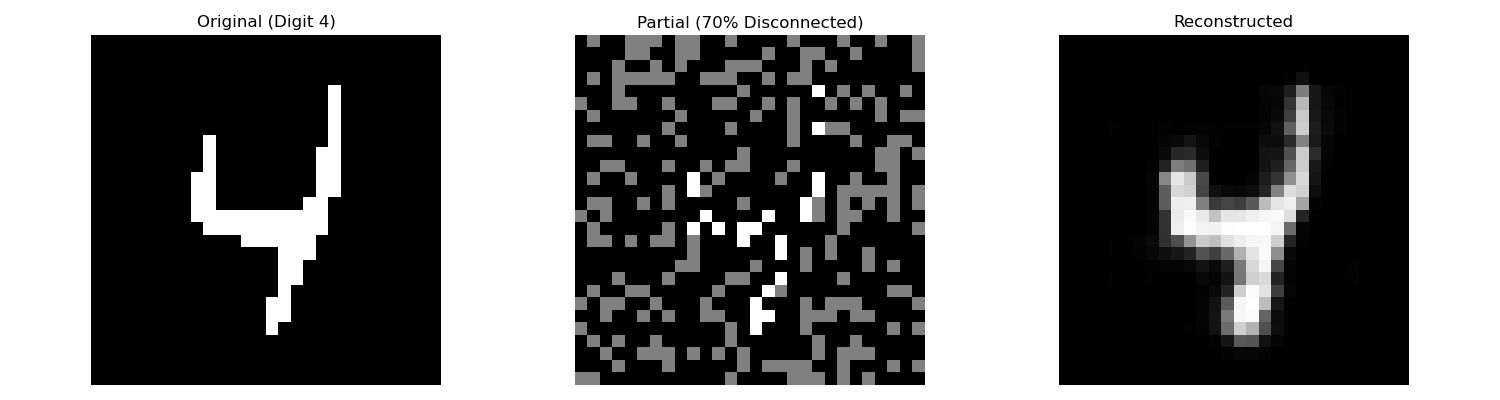
\includegraphics[width=0.9\textwidth]{sample_15.png}\\
    \emph{Figure (6-4) : Exemple d'image originale, image avec 70\,\% de pixels déconnectés et image reconstruite par l’Autoencoder.}\\
    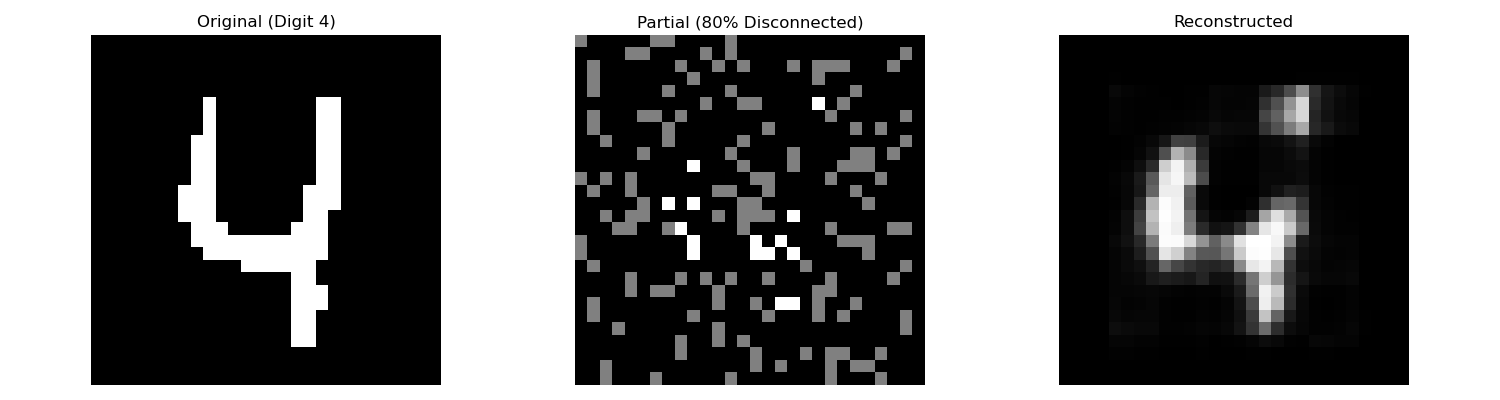
\includegraphics[width=0.9\textwidth]{sample_11.png}\\
    \emph{Figure (6-5) : Exemple d'image originale, image avec 80\,\% de pixels déconnectés et image reconstruite par l’Autoencoder.}\\

\end{enumerate}

\subsection*{Conclusion}
Dans cette partie du projet (section 6), nous avons appliqué un réseau de neurones convolutif de type Autoencoder sur le jeu de données MNIST afin de reconstituer les pixels manquants (jusqu’à 60\,\% de perte). Le modèle atteint en moyenne 94.7\,\% de précision pour la prédiction et la reconstruction. Toutefois, pour aborder des cas réels plus complexes, il faudra envisager des jeux de données bien plus étendus et des architectures plus sophistiquées.




\section{Algorithme MIS}
\subsection{Problématique}
Comment construire un ensemble indépendant maximal (MIS) de manière efficace et résiliente dans un environnement distribué ?
\subsection{Description}
L’algorithme MIS est essentiel pour de nombreuses tâches en réseaux distribués, notamment pour la gestion des ressources et la planification des transmissions.
\subsection{Implémentation et Résultats}




\section{Conception et Développement de l'Application}

\subsection{Introduction}
Dans le cadre de notre projet de fin d'études, nous avons développé une application web permettant de visualiser et de manipuler des graphes distribués. Cette application a été conçue en utilisant Django comme framework backend, HTML et JavaScript pour le frontend, et la bibliothèque GoJS pour la représentation graphique des graphes. Cette section décrit en détail la conception et le développement de l'application.

\subsection{Problématique}
Comment concevoir une interface interactive et intuitive pour la visualisation et la gestion des algorithmes distribués ?


\subsection{Architecture de l'Application}
L'application suit une architecture MVC (Modèle-Vue-Contrôleur) classique, où Django gère le modèle et le contrôleur, tandis que le frontend (HTML, JavaScript) gère la vue. GoJS est utilisé pour la partie graphique, permettant de créer, modifier et visualiser les graphes de manière interactive.

\begin{itemize}
    \item \textbf{Backend (Django)} : Gère la logique métier, la gestion des données, et les API nécessaires pour interagir avec le frontend.
    \item \textbf{Frontend (HTML, JavaScript)} : Gère l'interface utilisateur et les interactions avec l'utilisateur.
    \item \textbf{GoJS} : Bibliothèque JavaScript pour la création de diagrammes interactifs, utilisée pour représenter les graphes.
\end{itemize}

\subsection{Fonctionnalités de l'Application}
L'application offre plusieurs fonctionnalités clés pour la manipulation et la visualisation des graphes distribués :

\begin{itemize}
    \item \textbf{Création de Graphes} : Les utilisateurs peuvent créer des graphes en ajoutant des nœuds et des arêtes de manière interactive.
    \item \textbf{Visualisation des Graphes} : Les graphes sont affichés de manière claire et interactive, avec des options de zoom et de déplacement.
    \item \textbf{Manipulation des Graphes} : Les utilisateurs peuvent modifier les graphes en déplaçant des nœuds, en ajoutant ou en supprimant des arêtes, et en modifiant les propriétés des nœuds et des arêtes.
    \item \textbf{Sauvegarde et Chargement} : Les graphes peuvent être sauvegardés dans la base de données et rechargés ultérieurement.
    \item \textbf{Algorithmes sur les Graphes} : L'application permet d'exécuter des algorithmes de graphes (comme le parcours en largeur, en profondeur, ou la détection de cycles) et d'afficher les résultats.
\end{itemize}

\subsection{Développement du Backend avec Django}
Le backend de l'application a été développé en utilisant Django, un framework web Python. Django gère la logique métier, la gestion des données, et les API nécessaires pour interagir avec le frontend.

\begin{itemize}
    \item \textbf{Modèles} : Les modèles Django représentent les graphes, les nœuds, et les arêtes. Chaque graphe est composé de plusieurs nœuds et arêtes, stockés dans la base de données.
    \item \textbf{Vues} : Les vues Django gèrent les requêtes HTTP et renvoient les réponses appropriées. Elles sont utilisées pour créer, lire, mettre à jour, et supprimer des graphes.
    \item \textbf{API} : Des API REST ont été développées pour permettre au frontend d'interagir avec le backend. Ces API permettent de récupérer, créer, modifier, et supprimer des graphes.
\end{itemize}

\subsection{Développement du Frontend avec HTML, JavaScript et GoJS}
Le frontend de l'application a été développé en utilisant HTML pour la structure, JavaScript pour la logique interactive, et GoJS pour la représentation graphique des graphes.

\begin{itemize}
    \item \textbf{HTML} : La structure de base de l'interface utilisateur est définie en HTML. Cela inclut les formulaires pour créer et modifier des graphes, ainsi que la zone d'affichage du graphe.
    \item \textbf{JavaScript} : JavaScript est utilisé pour gérer les interactions utilisateur, comme le clic sur un nœud pour le déplacer, ou le clic sur un bouton pour exécuter un algorithme. Il est également utilisé pour interagir avec les API Django.
    \item \textbf{GoJS} : GoJS est une bibliothèque JavaScript puissante pour la création de diagrammes interactifs. Elle a été utilisée pour représenter les graphes de manière visuelle, avec des options de zoom, de déplacement, et de modification interactive.
\end{itemize}

\subsection{Intégration de GoJS}
GoJS a été intégré dans l'application pour fournir une interface graphique interactive pour les graphes. Voici comment GoJS a été utilisé :

\begin{itemize}
    \item \textbf{Initialisation du Diagramme} : Un diagramme GoJS est initialisé dans une zone HTML spécifique. Ce diagramme est configuré pour permettre l'ajout, la suppression, et la modification des nœuds et des arêtes.
    \item \textbf{Gestion des Événements} : Des gestionnaires d'événements sont définis pour gérer les interactions utilisateur, comme le clic sur un nœud pour le déplacer, ou le double-clic pour modifier ses propriétés.
    \item \textbf{Synchronisation avec le Backend} : Les modifications apportées au graphe dans GoJS sont synchronisées avec le backend Django via des appels API. Cela permet de sauvegarder les modifications dans la base de données.
\end{itemize}

\subsection{Exemple de Code}
Voici un exemple de code pour initialiser un diagramme GoJS et gérer les interactions utilisateur :

\begin{lstlisting}[language=JavaScript]
// Initialisation du diagramme GoJS
var $ = go.GraphObject.make;
var diagram = $(go.Diagram, "myDiagramDiv", {
    "undoManager.isEnabled": true,
    "click": function(e) {
        var node = e.diagram.selection.first();
        if (node instanceof go.Node) {
            console.log("Node clicked:", node.data.key);
        }
    }
});

// Définition du modèle de données
diagram.model = new go.GraphLinksModel(
    [
        { key: "Node1" },
        { key: "Node2" }
    ],
    [
        { from: "Node1", to: "Node2" }
    ]
);
\end{lstlisting}

\subsection{Conclusion}
L'application développée dans le cadre de ce projet permet de visualiser et de manipuler des graphes distribués de manière interactive. En combinant Django pour le backend, HTML et JavaScript pour le frontend, et GoJS pour la représentation graphique, nous avons créé une application robuste et facile à utiliser. Cette application peut être étendue avec des fonctionnalités supplémentaires, comme l'intégration d'algorithmes de graphes plus complexes, ou l'ajout de fonctionnalités de collaboration en temps réel.

\section{Expérimentations et Résultats}


\section{Applications et Perspectives}
Les applications possibles incluent :
\begin{itemize}
    \item Amélioration des protocoles P2P pour assurer une meilleure qualité de service (QoS).
    \item Extension aux systèmes massivement distribués.
    \item Développement de stratégies hybrides combinant redondance et prédiction.
\end{itemize}

\section{Conclusion}
Ce travail a permis de démontrer l’intérêt de l’apprentissage automatique pour améliorer la robustesse des algorithmes distribués face aux pannes de communication. Les résultats obtenus sont prometteurs et ouvrent la voie à de nouvelles approches pour optimiser les échanges d’informations dans des systèmes distribués.

\section{Annexes}
\begin{itemize}
    \item Code source et configurations.
    \item Compléments théoriques sur les algorithmes et les modèles utilisés.
\end{itemize}

\end{document}